\subsection{Hopfield networks}
Extreme cases of the noise parameter and number of iterations were tested on the \textit{hopdigit} example. Figures \ref{sec2_2} to \ref{sec2_3} show the results of 4 extreme experiments.
\bigbreak
Results in figures \ref{sec2_2} and \ref{sec2_4} show unstable states due to the limited number of iterations during the process. Hence the results did not converge. Nevertheless, the unstable states are relatively \textit{closed} to the stable states shown in figures \ref{sec2_1} and \ref{sec2_4}.
\bigbreak
Results in figures \ref{sec2_1} and \ref{sec2_3} after a bigger amount of iterations. It is clear that the noise (which implies the initial position of the input) affects the final result, a bigger noise (bigger distance from the target attractor) results in an unexpected result, as shown in figure \ref{sec2_3}.
\bigbreak
After an exhaustive iteration, no spurious states were found. 
\begin{figure}[!htbp]
\caption{Results of the \textit{hopdigit} function with noise=4 and numiter=10.}
\label{sec2_2}
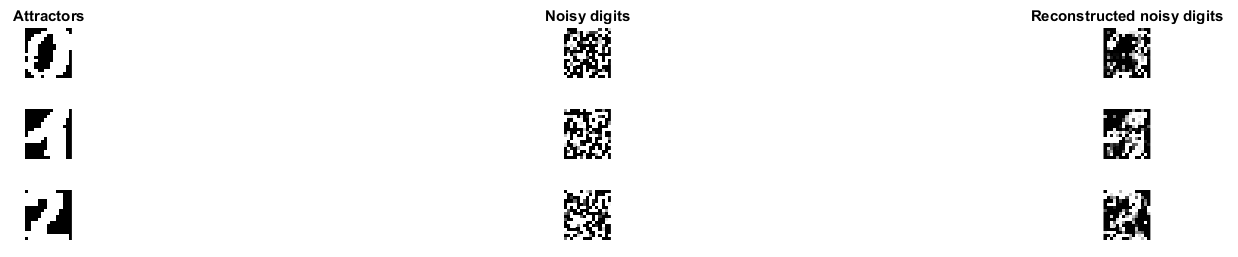
\includegraphics[width=\textwidth/2]{figures_2/hopdigit_4_10}
\centering
\end{figure}

\begin{figure}[!htbp]
\caption{Results of the \textit{hopdigit} function with noise=4 and numiter=100.}
\label{sec2_1}
\medbreak
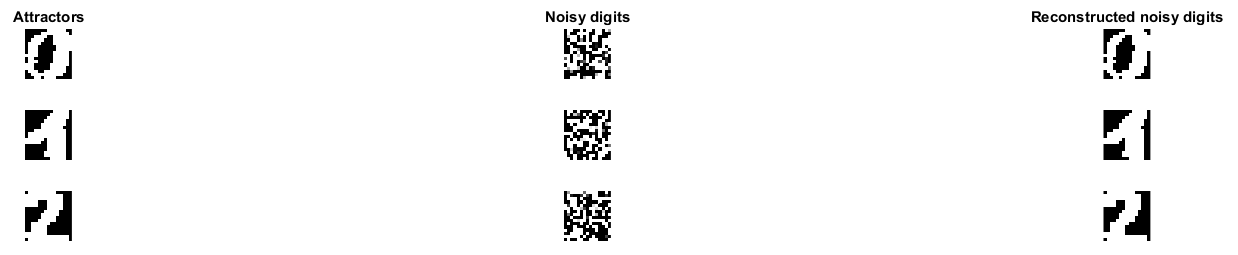
\includegraphics[width=\textwidth/2]{figures_2/hopdigit_4_1000_1}
\centering
\end{figure}

\begin{figure}[!htbp]
\caption{Results of the \textit{hopdigit} function with noise=100 and numiter=10.}
\label{sec2_4}
\medbreak
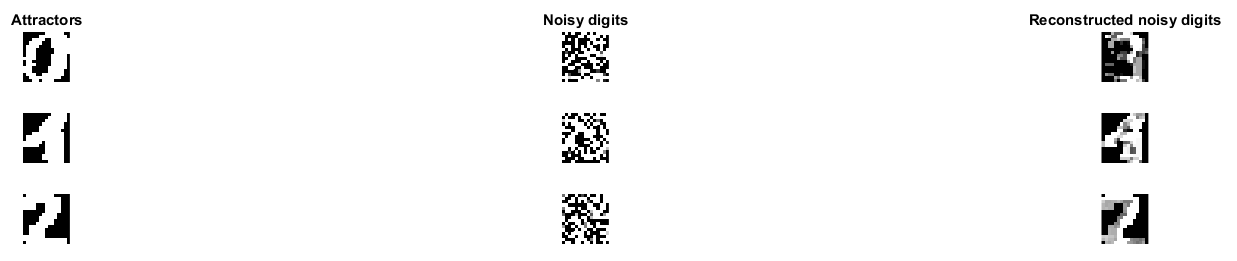
\includegraphics[width=\textwidth/2]{figures_2/hopdigit_10_10_1}
\centering
\end{figure}

\begin{figure}[!htbp]
\caption{Results of the \textit{hopdigit} function with noise=100 and numiter=100.}
\label{sec2_3}
\medbreak
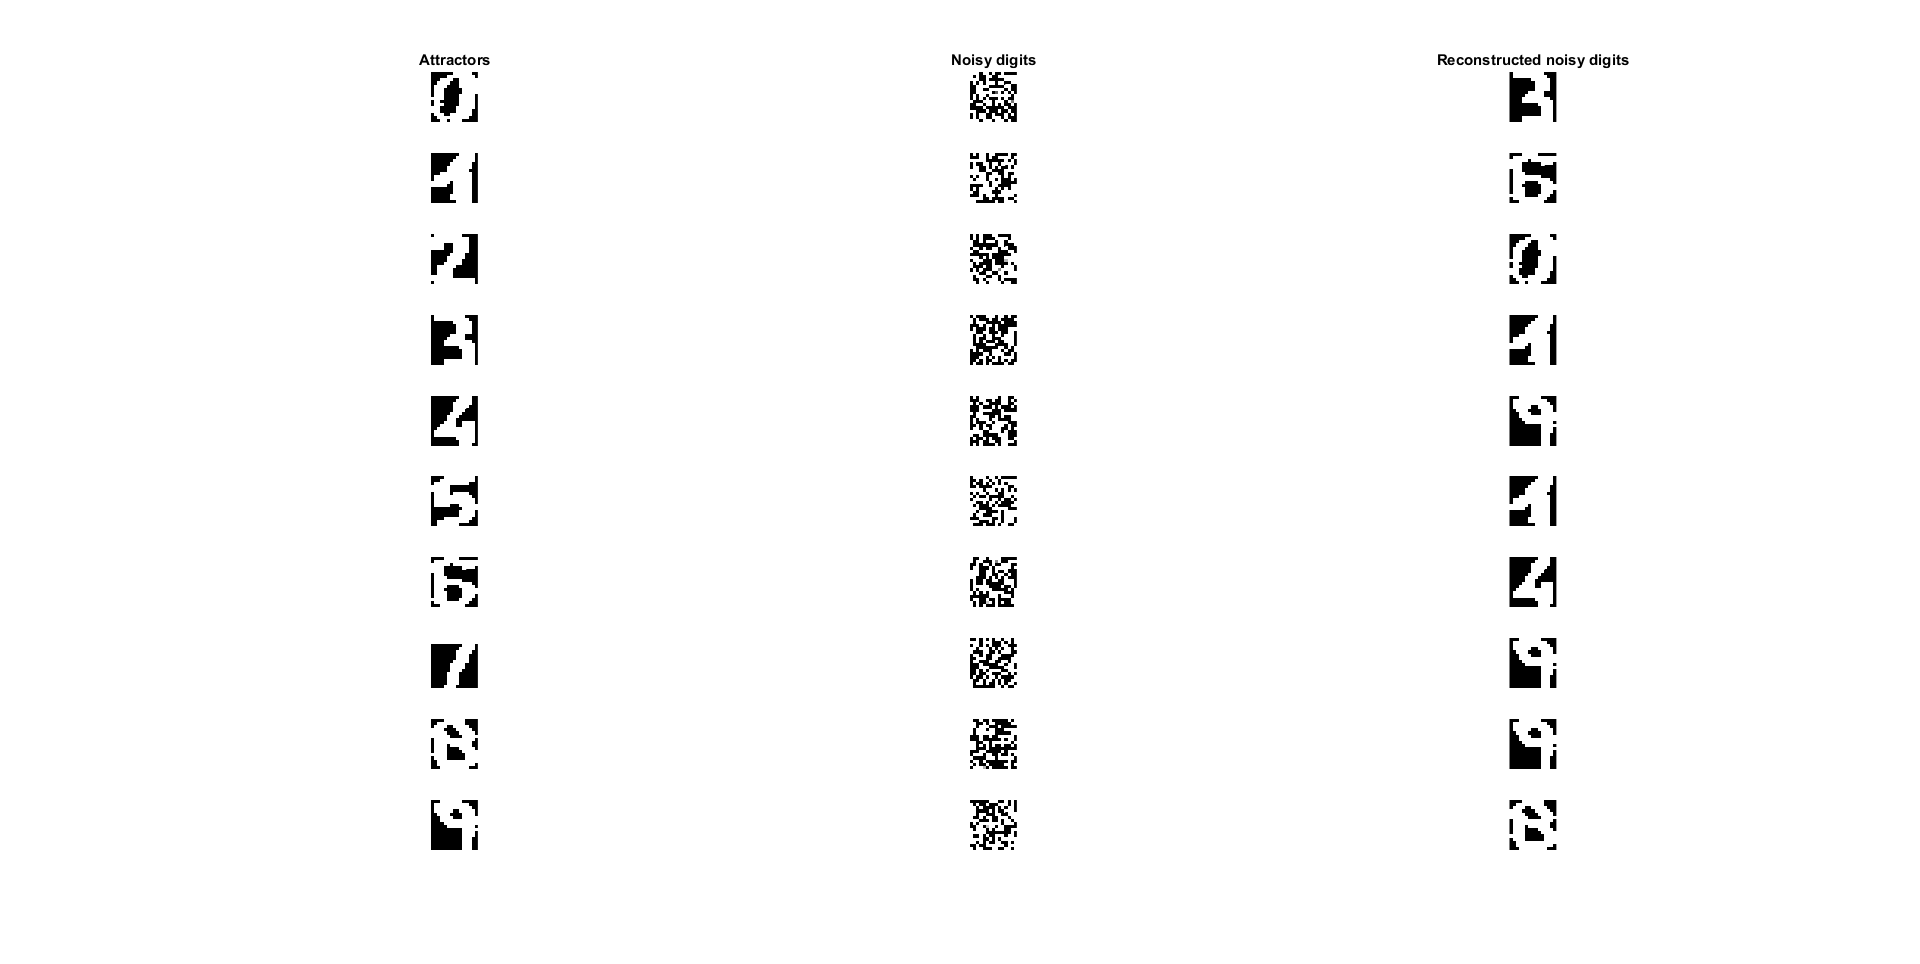
\includegraphics[width=\textwidth/2]{figures_2/hopdigit_100_100_2}
\centering
\end{figure}

\newpage

\subsection{Elman network}
Several experiments were done using different training points, epochs and neurons. To avoid a straightforward conclusion, three iterations per setup were run. Table \ref{s2_t1} shows the results.
\bigbreak
This experiments suggests that the number of neurons is a critical hyperparameter in the Helman network. There is a correlation between the recall and the neurons. There is a clearly negative effect when the number of neurons are increased. The number of epochs and training points increase the Recall and decrease the MSE in all the settings.


\begin{table}[!htbp]
\centering
\caption{Results of time-series predictions using an Elman network with different parameters}
\label{s2_t1}
\medbreak
\resizebox{\textwidth}{!}{
\begin{tabular}{c|c|c|c|c|c|c}
Training points & Epochs & Neurons & R1 - MSE1 & R2 - MSE2 & R3 - MSE3 & Avg R - Avg MSE \\\hline
300 & 100 & 50 & 0.8046 - 0.28165 & 0.86376 - 0.19918 & 0.82022 - 0.21337 & 0.82952 - 0.23140\\\hline
300 &  100 & 100 & 0.25316 - 0.74488 & 0.84409 - 0.22219 & 0.74083 - 0.24923 & 0.61269 - 0.40543\\\hline
300 &  100 & 500 & 0.066352 - 4.1895 & -0.37543 - 1.7456 & 0.36863 - 2.6571 & 0.01985 - 2.86406\\\hline

300 & 500 & 50 & 0.87958 - 0.17177 & 0.89757 - 0.14329 & 0.919663 - 0.13059 & 0.89893 - 0.44560\\\hline
300 &  500 & 100 & 0.83692 - 0.19721 & 0.77193 - 0.35833 & 0.8484 - 0.21193 & 0.81908 - 0.25582\\\hline
300 &  500 & 500 & 0.26619 - 2.4972 & 0.20328 - 2.8426 & 0.77812 - 0.33735 & 0.41586 - 1.89238\\\hline

300 & 1000 & 50 & 0.90988 - 0.1029 & 0.92109 - 0.089881 & 0.89314 - 0.14156 & 0.90803 - 0.11144\\\hline
300 & 1000 & 100 & 0.79292 - 0.34087 & 0.85052 - 0.23548 & 0.93913 - 0.095492 & 0.86085 - 0.22394\\\hline
300 & 1000 & 500 & 0.88905 - 0.13257 & 0.77324 - 0.2473 & 0.74208 - 0.37589 & 0.80145 - 0.25192\\\hline

500 & 100 & 50 & 0.91346 - 0.70402 & 0.89814 - 0.12147 & 0.86020 - 0.17218 & 0.89363 - 0.33255 \\\hline
500 &  100 & 100 & 0.31444 - 1.0704 & 0.73214 - 0.35368 & 0.75021 - 0.26852 & 0.59893 - 0.56346\\\hline
500 &  100 & 500 & 0.058904 - 4.2432 & 0.082859 - 2.4775 & -0.028816 - 1.9908 & 0.03764 - 2.9038\\\hline

500 & 500 & 50 & 0.66104 - 0.83886 & 0.77711 - 0.29763 & 0.82016 - 0.23519 & 0.75277 - 0.45722 \\\hline
500 &  500 & 100 & 0.88826 - 0.15023 & 0.7454 - 0.28408 & 0.8295 -0.24462 & 0.82105 - 0.22631 \\\hline
500 &  500 & 500 & 0.3947 - 2.0466 & 0.71847 - 0.30259 & 0.41324 - 2.136 & 0.50880 - 1.49506\\\hline

500 & 1000 & 50 & 0.96242 - 0.053706 & 0.94135 - 0.082144 & 0.8931 - 0.12993 & 0.93229 - 0.08859\\\hline
500 & 1000 & 100 & 0.81748 - 0.25344 & 0.89584 - 0.14696 & 0.82683 - 0.25421 & 0.84671 - 0.21820\\\hline
500 & 1000 & 500 & 0.54997 - 1.2887 & 0.88085 - 0.15332 & 0.9128 - 0.11874 & 0.78120 - 0.52015

\end{tabular}}
\end{table}